A unity gain feedback system with $K=1$ and its Bode plot are shown below. 
\begin{enumerate}
\item Based on clues from the Bode plot magnitude and phase, determine which of the Nyquist plots is correct.  (Note that arrows have been added to indicate directionality.)
\item Based on your answer to (a) and the Nyquist stability criterion, is the closed-loop system stable?
\end{enumerate}

\begin{center}
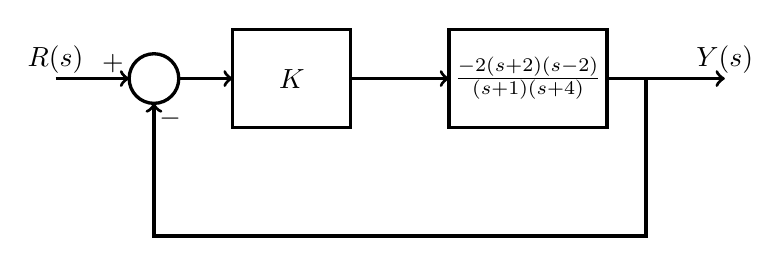
\begin{tikzpicture}[scale=1,inner sep=0pt,outer sep=0pt,very thick,
sysblock/.style={draw,rectangle,inner sep=2pt,minimum width=1.5cm,minimum height=1.25cm,very thick}]

\draw (1.25,0) node[draw,circle] (sum1) {$\rule{0pt}{18pt}$};
\draw (3,0) node[sysblock] (Kp) {$K$};
\draw (6,0) node[sysblock] (G) {$\frac{-2(s+2)(s-2)}{(s+1)(s+4)}$};

\draw[->] (0,0) node[above=2pt] {$R(s)$} -- (sum1.180) node[above left=2pt] {$+$};
\draw[->] (sum1.0) --   (Kp);
\draw[->] (Kp) -- (G.180);
\draw[->] (G) -- ++(2.5,0) node[above=2pt] {$Y(s)$};
\draw[->] (G) ++(1.5,0) -- ++(0,-2) -| (sum1.-90) node[below right=2pt] {$-$};
\end{tikzpicture}

\includegraphics[width=4in]{\mainfolder/LectureNotes/\lecturefolder/HomeworkProblems/Problem06part1.png}

\includegraphics[width=6in]{\mainfolder/LectureNotes/\lecturefolder/HomeworkProblems/Problem06part2.png}

\end{center}

